\documentclass{article}

\usepackage{graphicx}
\usepackage{tikz}
\usepackage{pgfplots}
\usepackage{hyperref}
\usepackage{listings}
\usepackage{indentfirst}
\usepackage{amssymb}
\usepackage{mathtools}
\usepackage{geometry}
\usepackage{float}
\geometry{
	a4paper,
	total={170mm,257mm},
	left=15mm,
	top=8mm,
	right=15mm,
	bottom=13mm
}
\lstset{
	frame=tb, 
	tabsize=4, 
	showstringspaces=false,
	numbers=left, 
	commentstyle=\color{green}, 
	keywordstyle=\color{blue}, 
	stringstyle=\color{red} 
}
\setlength{\parindent}{1.5cm}
\DeclarePairedDelimiter{\abs}{\lvert}{\rvert}

\author{Parfene Ioana, Panainte Alexandru, Donciu Codrin}
\title{\textbf{Fake news detection for Romanian}}

\begin{document}
	\maketitle
	
	\section{Introduction}
	\par This article documents the process of using several classifiers in order to identify fake news from Romanian news web sites. The algorithms are tested on different vectorization procedures, lengths of tokenized vocabularies and test data sizes. The sought after information pertains to the accuracy and time of each classification run.
	\subsection{Motivation}	
	Fake news as a term is defined as the deliberate spread of misinformation via traditional news media or via social media. Its purpose relates to manipulating the masses for political, social, economical or cultural purposes, creating panic or "trolling" as a way of satisfying one's ego or personal view of fighting against a particular moral concept present in current societal norms. It can start with satirical or sarcastic intentions, but snowball and spread at an out of control rate, slowly changing and adapting each time it is shared. Regardless of origin and intent, fake news can rapidly cause damage on a high scale and lasting repercussions. This project aims to take the concept of fake news detection, which is widely known and researched, and apply it to the Romanian language, which is a far less explored territory. 
	
	\section{Method}
	The process makes use of Romanian fake and true news articles scraped from real and satire news sites. The text is preprocessed through tokenization and stemming, vectorized and passed through several classifiers in order to find the one that yields the best accuracy and/or time. The detection method was researched through multiple articles and the chosen programming language is Python. As soon as these details were set, many articles were read, a lot of research was done, many tasks were created and a lot of steps were collected into a diagram.
	\begin{figure}[!h]
		\centering
		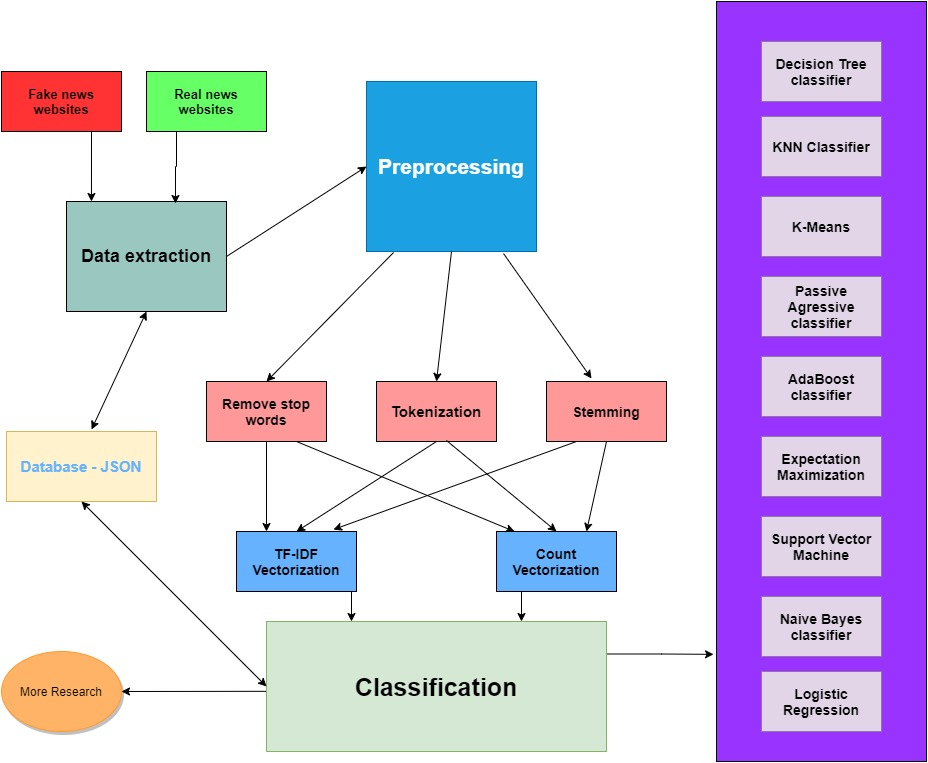
\includegraphics[width=12cm,height=12cm,keepaspectratio]{Pics/Diagram}
		\caption{Project Architecture}
	\end{figure}
	
	\subsection{Gathering Data}
	Finding sites that could be crawled and scraped was quite a daunting task. Real news are easy to find, there are countless organizations that have been existing for decades, in television, radio or newspaper formats. Fake news was, on the other hand, tricky. Nobody will write a bunch of false articles, admit to them being fake, then collect them together in a nice place to be found. True malicious or ill-intended posts were impossible to gather, so the next best thing was, logically, satire. Sarcastic news sites are a fraction of the news site pool, especially in Romania. This narrowed down the amount of data that could be collected, as the true corpus size had to be the same as the fake one. 
	\par There was also the question of how this restriction would apply into the real world. We used sarcastic articles and we tested them on more sarcastic articles. This can be very helpful against the rumor snowball effect that can lead to the creation of fake news, as well as the tone recognition problem faced by many people. Carefully crafted texts meant to destroy nations, create panic, mimic official and formal articles or exude authenticity would perform worse under this particular data set, but not go completely undetected. The topics chosen by the satire authors and their writings are more times than not meant to poke fun at pieces that circulate as fake news. They have their fair share of "true fake news" characteristics.

	\subsubsection{Web Sites}
	 The final corpus has 200 000 words, used across 1200 articles, equally spread between the two categories. There were 8 sites crawled and scraped, half for true news, half for satire.
	\begin{figure}[!h]
		\begin{tabular}{||c||l|l|l|l||l|l|l|l|||}
			\hline
			\textbf{Category} &  & \textbf{True} & \textbf{News}& & &\textbf{Fake} & \textbf{News} &  \\ \hline 
			\textbf{Web Sites} & \textbf{ProTV} & \textbf{Digi24} & \textbf{Libertatea} & \textbf{Realitatea} &\textbf{TNR} & \textbf{Cațavencii} & \textbf{7lucruri} & \textbf{TimpuriGrele} \\ \hline
			\textbf{Articles} & 124 &89 &91 & 108 &42 & 156 &502 & 96  \\ \hline 
			\textbf{Words} & 41,796 & 69,800 & 41,981 & 46,508 & 7,917 & 98,544 & 055,899 &37,690  \\ \hline 
		\end{tabular}
		\caption{\textbf{Web Site Corpus Distribution}}
	\end{figure} 

	\subsubsection{Crawling}
	The article link gathering was done through a process called "crawling", which means recursively finding and saving all the links found on a certain web page. Those saved links are used to continue the search, until no more are found or until a set limit. Some websites were tough to crawl, as they only advertised recent articles. This lead to a disproportionate distribution of total words obtained across all websites, but he main goal of finding equal amounts of true and fake news was met. The implementation was relatively easy, done using Python libraries.
	\subsubsection{Scraping}
	The actual downloading of the article text is called scraping. It involves using the HTML tags of the web sites in order to locate the content, which was quick as all the news sources fit into a pattern and only required one function with different inputs to scrape.
	
\subsection{Preprocessing}
	The articles had to be preprocessed before being passed through the classifiers. The first step was combining the title and content of each piece into one string. The second step was removing the stop words, then turning the string into individual words. The last process chosen in this particular implementation was stemming, which means reducing words to a short root that represents the differently-spelled versions of a certain notion.
	\subsubsection{Stop Words}
	This is the beginning of preparing the extracted texts for classifiers to properly label the data further down the line. Firstly, an extensive stop words list is needed, that we can identify in our texts and have them removed.\\After this, the actual process is a relatively easy task, as the app only needs to compare the raw data with this list of unnecessary words, and have them removed entirely.\\
	Multiple sources for choosing these stop words have been used, and they can be found in the references section of this document.
	\subsubsection{Tokenization}
Tokenization is the method of breaking down a large amount of text into smaller pieces called \textbf{tokens}. These tokens are extremely useful for pattern recognition and are used as a starting point for stemming and lemmatization. Tokenization here is also be used to replace sensitive data elements with non-sensitive ones.
We use the method \textbf{word\_tokenize()} to split a sentence into words. \\
For better text comprehension in machine learning applications, the performance of the word tokenizer in NLTK can be translated to a Data Frame.
	\subsubsection{Stemming}
	Stemming is the process of eliminating a word's suffix and reducing it to its \textbf{root word}. The main goal is to reduce each word's inflectional forms to a single base word, root word, or stem word. Inflection is the process of changing a word to convey different grammatical categories including tense, case, voice, aspect, person, number, gender, mood, animacy, and definiteness.
	For this project, we have employed the \textbf{Natural Language Toolkit} (NLTK) library and its \textbf{SnowballStemmer()} method, language parameter set on 'romanian' and stopwords ignore enabled, as the stopwords used were from a different library and not the NLTK native one.
	\begin{figure}[!h]
		\centering
		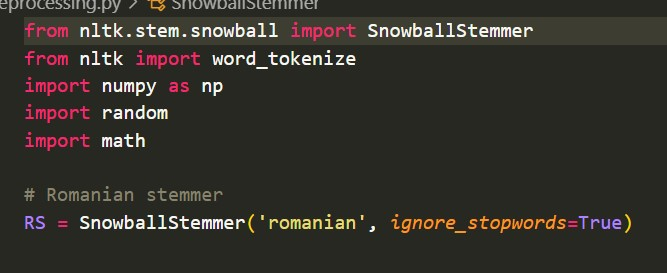
\includegraphics[width=12cm,height=12cm,keepaspectratio]{Pics/NLTK screenshot}
		\caption{Usage of SnowballStemmer}
	\end{figure}
	All of the data is stored in \textbf{.json} files after checking for satisfactory results with the stemming, tokenization and stop words removal processes. Further down the line, the classifiers we have implemented will have these files as input for their algorithms. 
	\subsection{Data Models}
	\subsubsection{Bag of Words}
	\subsubsection{TF-IDF}
	
	
	\subsection{Classifiers}
	\subsubsection{Naive Bayes}
	\begin{figure}[H]
		\begin{tabular}{||c||l|l|l|l||l|l|l|l||l|l|l|l||}
			\hline
			\textbf{Words} &  & \textbf{200} & & & &\textbf{1000} & & & & \textbf{19518} &  & \\ \hline 
			\textbf{Model} & \textbf{BoW} & \textbf{BoW} & \textbf{T-I} & \textbf{T-I} &\textbf{BoW} & \textbf{BoW} & \textbf{T-I} & \textbf{T-I} & \textbf{BoW} & \textbf{BoW} & \textbf{T-I} & \textbf{T-I}\\ \hline
			\textbf{Test} & \textbf{10\%} & \textbf{20\%} & \textbf{10\%} & \textbf{20\%} & \textbf{10\%} & \textbf{20\%} & \textbf{10\%} & \textbf{20\%} & \textbf{10\%} & \textbf{20\%} & \textbf{10\%} & \textbf{20\%} \\ \hline \hline  
			\textbf{Result} & 82.5\% & 82.9\% & 82.6\% & 82.9\% & 90.3\% & 89.7\% & 87.4\% & 86.6\% & 93.3\% & 93.3\% & 73.0\% & 71.8\% \\ \hline 
			\textbf{Time} & 0.01s & 0.01s & 0.01s & 0.01s & 0.09s & 0.08s & 0.05s & 0.06s & 1.76s & 1.67s & 0.98s & 1.08s \\ \hline 
		\end{tabular}
		\caption{\textbf{Naive Bayes}, Accuracy Table, \textbf{Average} out of \textbf{100} runs}
	\end{figure}
    
	\subsubsection{Passive Aggressive Classifier}
	\begin{figure}[H]
		\begin{tabular}{||c||l|l|l|l||l|l|l|l||l|l|l|l||}
			\hline
			\textbf{Words} &  & \textbf{200} & & & &\textbf{1000} & & & & \textbf{19518} &  & \\ \hline 
			\textbf{Model} & \textbf{BoW} & \textbf{BoW} & \textbf{T-I} & \textbf{T-I} &\textbf{BoW} & \textbf{BoW} & \textbf{T-I} & \textbf{T-I} & \textbf{BoW} & \textbf{BoW} & \textbf{T-I} & \textbf{T-I}\\ \hline
			\textbf{Test} & \textbf{10\%} & \textbf{20\%} & \textbf{10\%} & \textbf{20\%} & \textbf{10\%} & \textbf{20\%} & \textbf{10\%} & \textbf{20\%} & \textbf{10\%} & \textbf{20\%} & \textbf{10\%} & \textbf{20\%} \\ \hline \hline  
			\textbf{Result} & 83.0\% & 83.4\% & 84.3\% & 84.5\% & 93.1\% & 93.3\% & 93.5\% & 92.6\% & 94.3\% & 93.8\% & 94.2\% & 94.0\% \\ \hline 
			\textbf{Time} & 0.03s & 0.03s & 0.03s & 0.03s & 0.13s & 0.13s & 0.17s & 0.15s & 2.50s & 2.3s & 2.79s & 2.63s \\ \hline 
		\end{tabular}
		\caption{\textbf{Passive Aggressive Classifier}, Accuracy Table, \textbf{Average} out of \textbf{100} runs}
	\end{figure}    
    
	\subsubsection{Logistic Regression}
	\begin{figure}[H]
		\begin{tabular}{||c||l|l|l|l||l|l|l|l||l|l|l|l||}
			\hline
			\textbf{Words} &  & \textbf{200} & & & &\textbf{1000} & & & & \textbf{19518} &  & \\ \hline 
			\textbf{Model} & \textbf{BoW} & \textbf{BoW} & \textbf{T-I} & \textbf{T-I} &\textbf{BoW} & \textbf{BoW} & \textbf{T-I} & \textbf{T-I} & \textbf{BoW} & \textbf{BoW} & \textbf{T-I} & \textbf{T-I}\\ \hline
			\textbf{Test} & \textbf{10\%} & \textbf{20\%} & \textbf{10\%} & \textbf{20\%} & \textbf{10\%} & \textbf{20\%} & \textbf{10\%} & \textbf{20\%} & \textbf{10\%} & \textbf{20\%} & \textbf{10\%} & \textbf{20\%} \\ \hline \hline  
			\textbf{Result} & 86.1\% &85.9 \% & 85.5\% & 84.8\% &93.8\% &93.2\% &84.2\% & 82.9\% & 93.7\% &93.2 \% &72.1 \% &71.4\% \\ \hline 
			\textbf{Time} & 0.10s & 0.09s & 0.04s & 0.04s & 0.25s & 0.22s & 0.13s &0.11s & 3.98s & 3.84s & 1.86s & 2.14s \\ \hline 
		\end{tabular}
		\caption{\textbf{Logistic Regression}, Accuracy Table, \textbf{Average} out of \textbf{100} runs}
	\end{figure} 

	\subsubsection{K Nearest Neighbour}
	\begin{figure}[H]
		\begin{tabular}{||c||l|l|l|l||l|l|l|l||l|l|l|l||}
			\hline
			\textbf{Words} &  & \textbf{200} & & & &\textbf{1000} & & & & \textbf{19518} &  & \\ \hline 
			\textbf{Model} & \textbf{BoW} & \textbf{BoW} & \textbf{T-I} & \textbf{T-I} &\textbf{BoW} & \textbf{BoW} & \textbf{T-I} & \textbf{T-I} & \textbf{BoW} & \textbf{BoW} & \textbf{T-I} & \textbf{T-I}\\ \hline
			\textbf{Test} & \textbf{10\%} & \textbf{20\%} & \textbf{10\%} & \textbf{20\%} & \textbf{10\%} & \textbf{20\%} & \textbf{10\%} & \textbf{20\%} & \textbf{10\%} & \textbf{20\%} & \textbf{10\%} & \textbf{20\%} \\ \hline \hline  
			\textbf{Result} & 75.7\% & 75.3\% & 73.7\% & 73.4\% & 75.0\% & 74.2\% & 73.3\% & 73.0\% & 71.6\% & 71.1\% & 67.8\% & 66.2\% \\ \hline 
			\textbf{Time} &0.02s & 0.03s & 0.01s & 0.02s & 0.09s & 0.09s & 0.06s & 0.06s & 1.69s & 1.71s & 1.03s & 1.09s \\ \hline 
		\end{tabular}
		\caption{\textbf{K Nearest Neighbour(2 neighbours)}, Accuracy Table, \textbf{Average} out of \textbf{100} runs}
	\end{figure}

	\subsubsection{Support-vector machine}
	Support vector machines (SVMs) are a class of supervised learning methods for classification, regression, and identification of outliers. Some of the \textbf{advantages} of SVMs, that are relevant to our project, can be:
	\begin{itemize}
    \item it performs effectively in high-dimensional spaces.
    \item it is memory efficient since it uses a subset of training points (called support vectors) in the decision function.
    \item when the number of dimensions exceeds the number of samples, the method is still accurate.
    \end{itemize}
    \textbf{Disadvantages} of this method consist of:
    \begin{itemize}
    \item SVMs do not have probability estimates directly; these are estimated using a time-consuming five-fold cross-validation procedure.
    \item avoiding over-fitting when selecting Kernel functions and regularization terms is critical if the number of features is much greater than the number of samples.
    \end{itemize}
    Basically, SVM considers all of the data points and generates a line called a "Hyperplane" that separates the two groups: fake and true news. A "decision boundary" is created.

	\begin{figure}[H]
		\begin{tabular}{||c||l|l|l|l||l|l|l|l||l|l|l|l||}
			\hline
			\textbf{Words} &  & \textbf{200} & & & &\textbf{1000} & & & & \textbf{19518} &  & \\ \hline 
			\textbf{Model} & \textbf{BoW} & \textbf{BoW} & \textbf{T-I} & \textbf{T-I} &\textbf{BoW} & \textbf{BoW} & \textbf{T-I} & \textbf{T-I} & \textbf{BoW} & \textbf{BoW} & \textbf{T-I} & \textbf{T-I}\\ \hline
			\textbf{Test} & \textbf{10\%} & \textbf{20\%} & \textbf{10\%} & \textbf{20\%} & \textbf{10\%} & \textbf{20\%} & \textbf{10\%} & \textbf{20\%} & \textbf{10\%} & \textbf{20\%} & \textbf{10\%} & \textbf{20\%} \\ \hline \hline  
			\textbf{Result} & 86.1\% &85.9 \% & 75.5\% & 74.8\% &90.1\% &89.2\% &81.2\% & 79.9\% & 92.7\% &91.2 \% &90.1 \% &89.4\% \\ \hline  
			\textbf{Time} &0.32s & 0.33s & 0.31s & 0.32s & 1.09s & 1.09s & 1.06s & 1.06s & 20.69s & 20.71s & 15.03s & 16.09s \\ \hline 
		\end{tabular}
		\caption{\textbf{SVM}, Accuracy Table, \textbf{Average} out of \textbf{100} runs}
	\end{figure}

	\subsubsection{Decision Tree Classifier}
	Decision Trees (DTs) are a supervised learning system for classification and regression that is non-parametric. The aim is to learn basic decision rules from data features to build a model that predicts the value of a target variable. A tree is an approximation to a piecewise constant.
	\textbf{Advantages} of DTs:
\begin{itemize}
\item decision trees need less effort for data preparation during pre-processing than other algorithms.
\item the model is based on a white box. If a scenario can be observed in a model, boolean logic can easily clarify the situation.
\item even if the true model, from which the data were produced, violates some of its assumptions, it still performs well.
\end{itemize}
Some of the \textbf{disadvantages} of using Decision Tree classifier:
\begin{itemize}
\item as compared to other algorithms, a decision tree's calculation can become very complicated at times.
\item any minor change in the data will result in a significant change in the decision tree's structure, resulting in instability.
\item the training time for a decision tree is usually longer
\item because of the difficulty and time required, decision tree training is relatively costly
\end{itemize}
	\begin{figure}[H]
		\begin{tabular}{||c||l|l|l|l||l|l|l|l||l|l|l|l||}
			\hline
			\textbf{Words} &  & \textbf{200} & & & &\textbf{1000} & & & & \textbf{19518} &  & \\ \hline 
			\textbf{Model} & \textbf{BoW} & \textbf{BoW} & \textbf{T-I} & \textbf{T-I} &\textbf{BoW} & \textbf{BoW} & \textbf{T-I} & \textbf{T-I} & \textbf{BoW} & \textbf{BoW} & \textbf{T-I} & \textbf{T-I}\\ \hline
			\textbf{Test} & \textbf{10\%} & \textbf{20\%} & \textbf{10\%} & \textbf{20\%} & \textbf{10\%} & \textbf{20\%} & \textbf{10\%} & \textbf{20\%} & \textbf{10\%} & \textbf{20\%} & \textbf{10\%} & \textbf{20\%} \\ \hline \hline  
			\textbf{Result} & 80.6\% & 80.2\% & 80.9\% & 80.2\% & 88.2\% & 88.3\% & 87.1\% & 86.7\% & 89.6\% & 88.4\% & 87.2\% & 87.7\% \\ \hline 
			\textbf{Time} & 0.05s & 0.05s & 0.06s & 0.05s & 0.23s & 0.19s & 0.26s & 0.22s & 11.8s & 9.5s & 9.9s & 7.0s \\ \hline 
		\end{tabular}
		\caption{\textbf{Decision Tree Classifier}, Accuracy Table, \textbf{Average} out of \textbf{100} runs}
	\end{figure}
	
	\subsubsection{Ada Boost Classifier}
	An AdaBoost classifier is a meta-estimator that starts by fitting a classifier on the original dataset, then 
fits additional copies of the classifier on the same dataset, but adjusts the weights of incorrectly classified 
instances such that subsequent classifiers concentrate more on difficult cases. \\
\textbf{Advantages} of using this classifier:
\begin{itemize}
\item AdaBoost is often referred to as the strongest out-of-the-box classifier because it uses decision trees as poor learners.
\item it may be less prone to overfitting than other algorithms in certain situations.
\item individual learners can be slow, but as long as their output is better than random guessing, the final model will converge to a good learner.
\end{itemize}
\\
Among the \textbf{disadvantages} of this classifier, one that pertains to our project is:
\begin{itemize}
\item AdaBoost is vulnerable to outliers and noisy data.
When the data isn't easily amenable to a particular separation plane (with acceptable results based on the model objective. 
For example, weak learners must be better than guessing at random), making it more difficult for the meta-learner to converge to a strong learner without overfitting.
As a result, we can conclude that AdaBoost performs better when the dataset is free of outliers.
\end{itemize}
	\begin{figure}[H]
		\begin{tabular}{||c||l|l|l|l||l|l|l|l||l|l|l|l||}
			\hline
			\textbf{Words} &  & \textbf{200} & & & &\textbf{1000} & & & & \textbf{19518} &  & \\ \hline 
			\textbf{Model} & \textbf{BoW} & \textbf{BoW} & \textbf{T-I} & \textbf{T-I} &\textbf{BoW} & \textbf{BoW} & \textbf{T-I} & \textbf{T-I} & \textbf{BoW} & \textbf{BoW} & \textbf{T-I} & \textbf{T-I}\\ \hline
			\textbf{Test} & \textbf{10\%} & \textbf{20\%} & \textbf{10\%} & \textbf{20\%} & \textbf{10\%} & \textbf{20\%} & \textbf{10\%} & \textbf{20\%} & \textbf{10\%} & \textbf{20\%} & \textbf{10\%} & \textbf{20\%} \\ \hline \hline  
			\textbf{Result} & 86.3\% & 86.8\% & 86.2\% & 86.1\% & 93.5\% & 93.1\% & 92.8\% & 92.4\% & 93.5\% & 93.2\% & 92.9\% & 92.9\% \\ \hline 
			\textbf{Time} &0.2s & 0.2s & 0.3s & 0.3s & 1.3s & 1.1s & 1.5s & 1.3s &31.9s & 28.5s & 32.4s & 29.3s \\ \hline 
		\end{tabular}
		\caption{\textbf{Ada Boost Classifier}, Accuracy Table, \textbf{Average} out of \textbf{100} runs}
	\end{figure}
	
	\subsubsection{K-Means Classifier}
K-means is a centroid-based or distance-based algorithm in which the distances between points are calculated to allocate a point to a cluster.
Each cluster in K-Means is associated with a centroid. \\
Some of the \textbf{advantages} when employing usage of this classifier:
\begin{itemize}
\item relatively simple to implement.
\item scales well to large data sets.
\item guarantees convergence towards real/fake conclusion.
\item can warm-start the positions of centroids.
\item easily adapts to new examples.
\end{itemize}
\\
Among the \textbf{disadvantages} of this classifier:
\begin{itemize}
\item choosing K manually.
\item being dependent on initial values
\item clustering data pf varying sizes and density
\item scaling with number of dimensions
\end{itemize}
	\begin{figure}[H]
		\begin{tabular}{||c||l|l|l|l||l|l|l|l||l|l|l|l||}
			\hline
			\textbf{Words} &  & \textbf{200} & & & &\textbf{1000} & & & & \textbf{19518} &  & \\ \hline 
			\textbf{Model} & \textbf{BoW} & \textbf{BoW} & \textbf{T-I} & \textbf{T-I} &\textbf{BoW} & \textbf{BoW} & \textbf{T-I} & \textbf{T-I} & \textbf{BoW} & \textbf{BoW} & \textbf{T-I} & \textbf{T-I}\\ \hline
			\textbf{Test} & \textbf{10\%} & \textbf{20\%} & \textbf{10\%} & \textbf{20\%} & \textbf{10\%} & \textbf{20\%} & \textbf{10\%} & \textbf{20\%} & \textbf{10\%} & \textbf{20\%} & \textbf{10\%} & \textbf{20\%} \\ \hline \hline  
			\textbf{Result} & 8.4\% & 15.2\% & 15.9\% & 12.1\% & 12.3\% & 13\% & 13.9\% & 11.9\% & 10.4\% & 12.8\% & 14.6\% & 18.5\% \\ \hline 
			\textbf{Time} &0.1s & 0.1s & 0.2s & 0.2s & 0.5s & 0.4s & 0.5s & 0.5s & 7.8s & 7.1s & 7.7s & 6.7s \\ \hline 
		\end{tabular}
		\caption{\textbf{K-Means Classifier}, Accuracy Table, \textbf{Average} out of \textbf{100} runs}
	\end{figure}

	\section{Results}
	
	\section{Conclusion}
	
	\begin{thebibliography}{9}

		
	\end{thebibliography}  
\end{document}
